\documentclass[a4paper,12pt,oneside,final]{extbook}

\usepackage[utf8]{inputenc}
\usepackage[T1]{fontenc}
\usepackage{graphicx}
\usepackage{times}
\usepackage[english,swedish]{babel}
\usepackage[export]{adjustbox}
\usepackage{geometry}
\usepackage{array}

\geometry{
 margin=20mm
} 

\usepackage{fancyhdr}

\usepackage{titling}
\title{Individuell rapport, TNM094}
\author{Daniel Olsson\\Flerreglarsspel}

\frenchspacing
\setlength{\parindent}{0pt}
\parskip 5pt

\usepackage{color}
\definecolor{rltred}{rgb}{.5,0,0}
\definecolor{rltgreen}{rgb}{0,.5,0}
\definecolor{rltblue}{rgb}{0,0,1}

\usepackage[pdftex,
 colorlinks=true,
 urlcolor=rltblue,       % \href{...}{...} external (URL)
 filecolor=rltgreen,     % \href{...} local file
 linkcolor=rltred,       % \ref{...} and \pageref{...}
 citecolor=rltgreen,     % \cite{...}
 pdftitle={},
 pdfauthor={},
 pdfsubject={Projektrapport, TNM094},
 pdfkeywords={},
 pdfpagemode=,
 pdfstartview=FitH,
 bookmarks=true,
 bookmarksopen=false,
 bookmarksnumbered=true
        ]{hyperref}


\begin{document}

\pagestyle{empty}
\thispagestyle{empty}

\frontmatter

\maketitle

\pagestyle{fancy}

\chapter{Sammanfattning}

\textcolor{red}{
En sammanfattning ska kort och koncist beskriva och motivera det studerade problemet, metoden
samt resultat och slutsatser. Arbetets bidrag till huvudområdet ska tydligt framgå. Vad är det rapporten
säger om huvudområdet som vi inte visste tidigare?
Sammanfattningens längd växer med längden på rapporten. I en rapport av denna typ kan den vara tre
stycken lång: ett inledande motiverar arbetet och beskriver bakgrund, ett beskriver redogörelsen och
ett beskriver analys och slutsatser. Sammanfattningen innehåller inga referenser eller ekvationer}


\tableofcontents

\cleardoublepage
% \phantomsection
\addcontentsline{toc}{chapter}{\listfigurename}
\listoffigures

\cleardoublepage
% \phantomsection
\addcontentsline{toc}{chapter}{\listtablename}
\listoftables

\mainmatter

\chapter{Inledning}
\label{ch:inledning}

Processen för att utveckla ett system är ofta komplex och lång. Det finns därför många olika metodiker som utvecklare kan jobba enligt för att få processen att bli mer överblickbar, redundant och anpassningsbar. 

\section{Bakgrund}
Olika arbetsprocesser lämpar sig för olika sorters av projekt och det är därför viktigt att analysera varje projekt var för sig för att se vad som lämpar sig bäst. En fel metodutveckling kan få ödesdigra effekter i form av overhead och kanske till och med ett nedlagt projekt.
\section{Syfte}

Syftet med detta arbete är att analysera och rekommendera en passande utveckling plan för ett projekt. Detta innebär att ge förslag på utvecklingsmetodik, systemartitektur och projekthantering. Planen är en rekommendation och kan ändras under projektets gång.

Projektet innebär att slutprodukten skall vara ett spel där flera externa knappar och spakar används för att styra och kontroller olika aspekter av spelmiljön.  


\section{Frågeställning}
För att kunna analysera vilken arbetsprocess som passar utvecklingsteamet bäst måste det definieras vad det är som eftersträvas med en vis arbetsprocess. Det som eftersträvas är minskad tidsåtgång och högre kvalitet på slutprodukten och detta kan formuleras med följande frågeställningar: 
\begin{itemize}
	\item Vilken utvecklingsmetodik ger minst overhead?
	\item  Går de att sammankoppla de fysiska reglagen med en spelmotor? Dvs vilka redskap och anslutningar behövs det för att få en signal från ett externt input till en spelmotor där den kan behandlas

\end{itemize}

\textcolor{red}{Observera att en specifik frågeställning nästan alltid ger ett bättre arbete än en generell frågeställning
(det är helt enkelt mycket svårare att göra något vettigt av en generell frågeställning). Det är också
fördelaktigt att inte bara skriva frågan, utan förtydliga i ett par meningar vad som menas med frågan
och hur den kan besvaras.
Det bästa sättet att få till en riktigt bra och specifik frågeställning är att göra en noggrann teorigenomgång
och sätta sig in i relaterad forskning och praktik. Då får man idéer och terminologi på köpet}





\section{Avgränsningar}
Inga avgränsningar har gjort för detta arbetet.


\chapter{System och tekniska lösningar}
I detta kapitel diskuteras tekniska lösningar för projektet och eventuella tredjepart programvara.

\section{Grundläggande, initiala krav och systembegränsningar}
Slutprodukten skall vara ett spel som skall vara lärande för barn men samtidigt kul och utmanande. Spelet skall stå i en utställning på visualations center i Norrköping och detta ställer en del krav på systemet. I samarbete med kunden tog en kravlista fram över slutprodukten vilket kan ses i sitt fullo i appendix \ref{Kravspecifikation}. De viktigaste punkterna kan ses nedan.

Slutprodukten skall:
\begin{itemize}
	\item minst använda sig av 3 externa knappar och 1 extern spak.
	\item vara spelbar för användare från 6 år.
	\item kräva minst 2 spelare.
	\item innehava ett tema om rymden eller programmering.
	\item vara lättmonterad.

\end{itemize}

Inga övre krav på användare finns då detta begränsas av antalet knappar som kommer implementeras vilket kan ändras under projektes gång. 

\section{Målplattform}

Projektet utvecklas för Windows 10 och ingen vikt kommer ges till att få spelet att bli bakåt kompatibelt. Detta är för att spelet är en del av en utställning och kommer därmed levereras med tillhörande hårdvara inklusive dator. 

Utvecklingsteamet kommer använda sig av en extern spelmotor. Detta är på grund av projektets storlek inte gör det hållbart att utveckla en spelmotor och utvecklingsteamet har inga framtida planer på spel så kostnaden för utvecklingen av en extern spelmotor kan inte delas på flera projekt. De spelmotorer som är intressanta är:
  
\begin{itemize}
	\item Unreal Engine 4
	\item Unity3D

\end{itemize}

 Valet mellan spelmotorerna grundar sig i en fundamental grundpelare som måste uppfyllas vilket är att motorn kan hantera externa input från hårdvara. Då båda motorerna klarar detta så valdes Unity3D då dess inlärningskurva är mycket bättre. 

\section{Grundläggande system-arkitektur}
Systemet som skall utvecklas kan grovt delas in i 3 delar:
\begin{itemize}
	\item Visualisering
	\item Inmatning
	\item Spellogik
\end{itemize}
Flödet som sker mellan dessa är sker alltid framåt. Visualisering ger data till användaren som ger nya kommandon via inmatningen som sedan behandlas av spellogiken och därefter uppdaterar visualiseringen. Detta system liknar strukturen för modell view controller(MVC)\cite{Design} och det är den strukturen som används för detta system på den högsta nivån. 



\begin{figure}[h]
	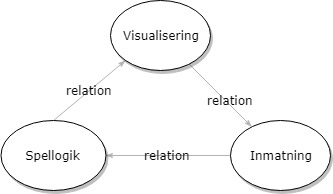
\includegraphics[width=0.5\textwidth, center]{System.jpg}
	\caption{Systemet tre stora objekt som samarbetar}
	\label{fig:System}
\end{figure}

Fördelar med denna struktur är att det är enklare att hitta fel i systemet och programkoden blir enklare att läsa då koden blir mer linjär och flödet är alltid riktat åt ett håll så som ses i \ref{fig:System}.

Visualiserings och spellogik objekten byggs upp i Unity3D och skrivs i C-sharp. Inmatnings objekten kommer handskas både i Untiy3D och en arduino. På arduinon skrivs koden i C och kommer endast hantera de externa kontrollernas  

\section{Standarder}



\textcolor{red}{Här beskrivs de standarder som systemet behöver följa, såsom filformat, protokoll eller andra gränssnitt.
Beskriv också vilka tredjeparts-APIer som kommer att användas för att göra detta.}

\section{Utvecklings-miljö}

I projektets utvecklingsfas kommer flera olika verktyg användas för att bygga och hantera slutprodukten.

Unity3D kommer användas för spelprogrammeringen och som leveleditor. Det är från Unity3D som spelet kommer kopileras från.

3DSmax kommer användas till modellering av alla spelmodeller.

Photoshop kommer användas till tillverkning av texturer.

Arduino Software kommer användas till programmeringen av Arduino.

Git kommer användas till versionshantering


\chapter{Projekthantering}

\textcolor{red}{Här beskrivs de övergripande teknikerna som övervakar och styr samarbetet inom projektet.}

\section{Utvecklingsmetodik}

\textcolor{red}{Beskriv och motivera här den övergripande strukturen, utvecklingsmetodiken eller metodikerna, som
	valts för projektet. Här ska bara grundläggande principer och motivering diskuteras. Detaljer diskuteras
	och motiveras under respektive avsnitt.
}

\section{Organisation}

\textcolor{red}{Här beskrivs vilka som ingår i projektet, både utvecklare och externa intressenter, deras ansvarsfördelning
	(och eventuellt hur den är planerad att förändras över tid) och eventuella arbetsgrupper och
	vilka syften och uppgifter dessa har.}

\section{Tidsplan}

\textcolor{red}{Beskriv, diskutera och motivera tidsplan för hela projektet, sprints, möten och milestones, inklusive
tid för planering och leverans.}

\section{Milestones och leverabler}

\textcolor{red}{Mer detaljerad beskrivning och motivering av milestones och leverabler, såsom rapporter, prototyper
och färdigt system.
}


\chapter{Rutiner och principer}

För att öka produktiviteten och samarbetet mellan alla utvecklare sätts rutiner upp. Dessa skall hjälpa att all kod och dokument följer ett särskilt mönster så att det inte blir misskommunikation mellan utvecklare.

\section{Mötesprinciper och rutiner}

Det kommer ske tre olika sorters möten och de är veckomöte, sprintmöte och scrummöte.  

Veckomöte är ett möte som infaller varje måndag klockan 08:15 för att säkerställa att all vet vad de ska göra den kommande veckan samt att påminna om eventuella kundmöten. Detta mötet skall ta ungefär 30 min.

Under sprintmötet bestämts vad som skall ske under nästa sprint och vad som skall färdigställas. Arbetsuppgifter delas ut bland de ansvariga utvecklarna som sedan delar ut de till sina utvecklargrupper. Detta mötet är beräknat till ca 60 min.

Scrummöterna sker i varje utvecklingsgrupp och där tas problem upp och diskuteras hur långt alla har kommit med sprinten.  Detta mötet är beräknat till ungefär 5 min.

\section{Kravhantering och -sårning}

\textcolor{red}{Beskriv hur gruppen arbetar med kravhantering och -spårning och vilket teknikstöd som kommer att
användas.}
\textcolor{red}{Här beskrivs också hur projektet säkerställer synkronisering mellan intressenternas behov och genomförandet.}


\section{Versionshantering, -system och rutiner}
Versionhantering är en viktigt pelare i ett projekt för att enklare kunna se vem som gjorde vad och gå tillbaka till gamla versioner. I detta projekt kommer Git användas som versionhanteringsprogram tillsammans med en extern server. Den externa serven kommer ligga på Gitlab. Valet att ha den externa servern på Gitlab grundar sig på tidigare licenser.

För att undvika konflikter och trasig kod så skall några få riktlinjer följas:
\begin{itemize}
	\item Alla commitments skall kommenteras kort. Nya tillägg skall kommenteras vad de gör och ändringar på gammal kod kommenteras vad de har ändrats. 
	\item Master branchen skall alltid innehålla fungerande kod, alla ändringar görs på en egen branch som sedan mergar in till mastern när den fungerar.
	\item Alla namn på branches skall innehålla i namnet vad som utvecklas och namn på ansvarig utvecklare. Stilen på namnet är \textit{Process\_Namn} och ett exempel kan se ut \textit{WrapperInput\_Daniel}.
	\item När en branch är fungerande skall alla test tas bort och branchen mergas in i mastern och sedan skall alltid branchen raderas om allt arbete på den är klar.
	\item Branches på branches behöver inte ha en ansvarig utvecklare i namnet. 
\end{itemize}

Dessa punkter är riktlinjer och skulle ett special dyka upp så skall detta diskuteras på ett möte.


\section{Arkitektur- och programdesign, standarder och rutiner}

\textcolor{red}{Beskriv hur gruppen arbetar med arkitektur och programdesign.}
\section{Dokumentationsprinciper och rutiner}
Dokumentation är en viktig del för att underlätta förståelse mellan utvecklare. Nedan beskrivs riktlinjerna för dokumentation.

\subsection{Programkod}
Programkod skall kommenteras på två olika ställen. En kommentar i toppen på varje fil och en över varje funktion. Kommentaren i toppen på varje fil skall innehålla:
\begin{itemize}
	\item Namnet på ansvarig utvecklare. Det menas med utvecklaren som är ansvarig för området och inte utvecklaren som har skrivit koden.
	\item Eventuella licenser
	\item Evuentuella tredjeparts-APIer som används.
	\item Kort sammanfattning vad filen gör.
\end{itemize}
All kommentering skall ske i Engelska.
\subsection{Möten}
Alla veckomöten skall dokumenteras enligt en fördefinerad mall som kan ses i bilaga \ref{protokoll}. De dagliga scrum mötena dokumenteras kortfattat i en textfil som lägg på samma server som all kod och hanteras av git. All dokumentation från möten sker på svenska.
\subsection{Slutproduktion}
Slutprodukten som är ett spel kommer dokumenteras på två sätt. En dokumentation kommer ske direkt i spelet iform av en introduktion till spelet och den andra dokumentationen är en manual hur slutprodukten skall kopplas samman. 

Indroduktionen i spelet kommer skrivas direkt i Unity3D och skall fokusera på att ge en grafisk handledning istället för text. Informationen ges på de språket som användaren har valt att spela i.

Manualen kommer skrivas i Latex och kommer innehålla en stegvis beskrivning på hur alla tillbehör sätt tillsammans samt hur slutprodukten installeras. Felsökning kommer även inkluderas i manualen. Manualen skrivs på Engelska.

\section{Kvalitetssäkring}

\textcolor{red}{Beskriv hur gruppen arbetar med kvalitetssäkring av programkod (granskning och testning) och vilket
teknikstöd som kommer att användas.
}

\chapter{Analys och diskussion}

\textcolor{red}{Det är här ni analyserar och diskuterar arbetet. I diskussionskapitlet ska man explicit referera till både
andra avsnitt i rapporten och externa källor som är relevanta för diskussionen.
}


\section{Resultat}

\textcolor{red}{Finns det något i resultaten som står ut och behöver analyseras och kommenteras? Vad säger teorin
om vad resultaten egentligen betyder? Finns det något i resultaten som är oväntat baserat på teori och
andra källor, eller stämmer det bra överens med vad man teoretiskt kunde förvänta sig?
}
\section{Arbetet i ett vidare sammanhang}

\textcolor{red}{Det ska ingå ett stycke med en diskussion om etiska och samhälleliga aspekter relaterade till arbetet.
Detta är viktigt för att påvisa professionell mognad samt för att utbildningsmålen ska kunna uppnås.
Om arbetet av någon anledning helt saknar koppling till etiska eller samhälleliga aspekter ska detta
explicit anges i stycket Avgränsningar i inledningskapitlet.
Exempel på samhälleliga eller etiska aspekter är människors liv och hälsa, samhällets funktionalitet,
demokrati, rättssäkerhet och mänskliga fri- och rättigheter, miljö och ekonomiska värden samt
nationell suveränitet. Inom planering av/och systemutveckling kan det exempelvis handla om arbetsbelastning,
ekonomisk kompensation, uppdelning mellan arbetstid och fritid, könsdiskriminering eller
annan form av diskriminering, programvarans användning i terrorism, kärnvapen, miljökopplad industri
eller demokratisk utveckling.}

\chapter{Slutsatser}

\textcolor{red}{I detta kapitel ska en återkoppling till syfte och frågeställningar ske. Har syftet uppnåtts och vad blev
svaret på frågeställningarna? Varje frågeställning kan få ett eget avsnitt för att tydliggöra strukturen.
Här ska också arbetets konsekvenser för berörd målgrupp och eventuellt för forskare och praktiker
beskrivas. Man kan också ha ett stycke eller avsnitt om framtida arbete där man beskriver vad man
skulle vilja göra om man hade mer tid eller som rekommendationer för framtida studier eller exjobb.
Om man har ett sådant stycke är det dock viktigt att det är konkreta och väl genomtänkta förslag som
presenteras, snarare än vaga idéer}


\bibliographystyle{vancouver}
\bibliography{referenser}

\addcontentsline{toc}{chapter}{Litteraturförteckning}

\pagestyle{empty}

\appendix

\chapter{Kravspecifikation}\label{Kravspecifikation}
\begin{center}
	\begin{tabular}{ | m{5em} | m{30em}| } 
		\hline
		Krav nr 1& Systemet skall minst använda sig av 3 externa knappar och 1 extern spak.   \\ 
		\hline
		Krav nr 2 & Systemet skall vara engagerande.  \\ 
		\hline
		Krav nr 3 & Systemet skall kunna brukas av en sexåring. \\ 
		\hline
		Krav nr 4& Systemet skall kräva minst två spelare för att vara spelbart. \\ 
		\hline
		Krav nr 5 & Systemet skall inte ge negativa responser vid fel utan ge konstruktiv kritik till användaren. \\ 
		\hline
		Krav nr 6 & Systemet skall inte innehålla ett traditionellt poängsystem. \\ 
		\hline
		Krav nr 7& En användare skall kunna lära sig kontrollerna för systemet under 2 minuter. \\ 
		\hline
		Krav nr 8 & Systemet skall öka svårighetsgrader så att det är svårt att bemästra systemet. \\ 
		\hline
		Krav nr 9 & Systemets skall ha rymdtema eller programmeringstema. \\ 
		\hline
		Krav nr 10& Systemet får inte manipulera projektionsvägen. \\ 
		\hline
		Krav nr 11& Systemet skall använda grafiska hjälpmedel för att visa knappar och spakars funktionalitet.  \\ 
		\hline
		Krav nr 12& Systemet skall gå att montera för en normalteknisk person på ca 2h. \\ 
		\hline
		Krav nr 13& Systemet skall kunna användas dagligen under 2 år utan att behöva repareras \\ 
		\hline
		Krav nr 14 & Systemet skall kunna skalas om till rum i olika storlekar. Minsta storlek på rum är 2x2 meter. \\ 
		\hline
	\end{tabular}
\end{center}


\chapter{Protokoll mall}\label{protokoll}

\end{document}